% Question 3

\begin{itemize}
    \item[(a)] We have the following R plot of various error curves:
    \begin{figure}[!ht]
        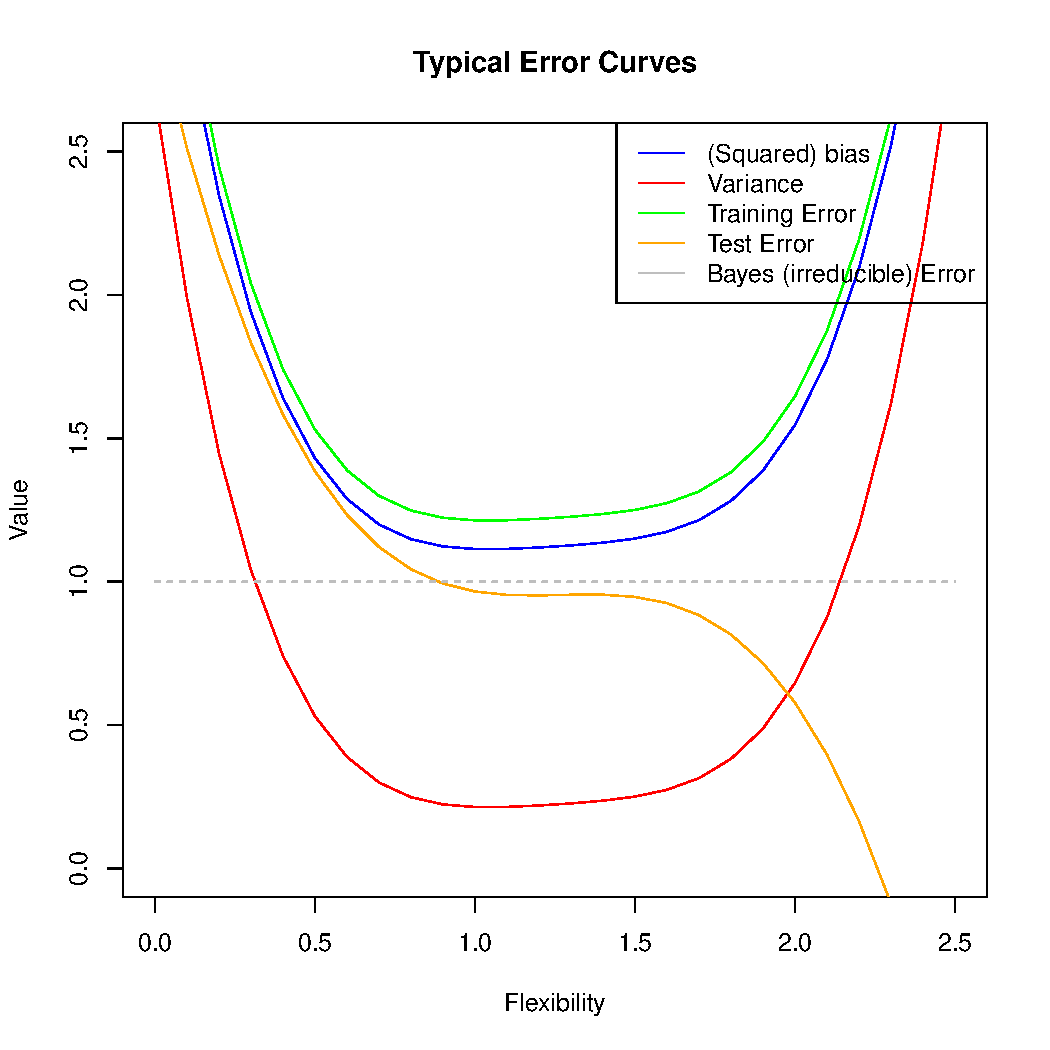
\includegraphics[scale=0.6, center]{./plots/ex2_3_a.pdf}
        \caption{
            Typical (squared) bias, variance, training error, test error, and Bayes 
            (irreducible) error
        }\label{fig:figure1}
    \end{figure}
    Arbitrary polynomials of the appropriate degree were used to generate these 
    plots, since they are approximations, using the following script:
    \begin{verbatim}
    \end{verbatim}
\end{itemize}
